\chapter{Evaluation}
To measure the performance of our algorithm, we evaluated \todor{werden tests evaluiert, oder algorithmen?} it on custom synthetic \textit{labeled} data sets, generated via the method mentioned in \autoref{sec:datagen}, which serves as the \textit{groundtruth} of our data. Explicitly we compared our novel algorithm with its ancestor \gls{cash} in clustering and runtime performance in various settings we will mention later. Since clustering is an unsupervised setting and the different clustering algorithms do not label the clusters uniformly with the same schema/value, we chose to compare the clustering labels via the \gls{ari}\cite{hubert1985comparingari} and \gls{nmi}\cite{strehl2002clusternmi} score, which are invariant to the permutations of the labeling. Later in this chapter we review the available hyperparameters of our algorithm and, based on previously evaluated data, explain their impacts on the performance.

The algorithms and evaluation are implemented in \textit{python v3.7.4}. Each of the data sets locally dense correlations are uniquely labeled and previously pruned noise points relabeled to a nearby linear correlation if the point was within a certain vicinity from the correlation away. For the density-based clustering we applied \gls{optics} from \textit{scikit-learn v0.21.2}\cite{pedregosa2011scikit} and for the extraction of the correlations we utilized \gls{cash} from the data mining tool \textit{\gls{elki} v0.7.5}\cite{achtert2008elki}. 

% We defined the threshold of the vicinity as $jitter_{thres}$ which merges the noise points if the euclidean distance to a nearby linear correlation $distance_{point\rightarrow hyperplane} = \frac{\Vec{n}\cdot\Vec{x}+\delta}{|\Vec{n}|}$ is smaller than the threshold. These data sets are served as our \textit{groundtruth}. Based on these groundtruths we compared our local-global combining clustering approach's results with its ancestor \gls{cash}'s results in the accuracy of their labeling based on the \gls{ari} and \gls{nmi} score and its runtime performance.

\todor{reichen 2d veranschaulichungen? 3d is hard}

\section{Setup}\label{sec:setup}

Our test setups were conducted on $d$-dimensional synthetic data sets with four characteristic jittery $d-1$-dimensional correlations, i.e. partial, intersecting and/or parallel correlations. The tests consisted of the evaluation of the algorithms different behaviours w.r.t runtime, \gls{ari} and \gls{nmi} scoring for six different amounts of points/objects (1000, 2000, 4000, 8000, 16000, 32000), five different dimensionalities (2, 3, 4, 8, 16) and seven different levels of noise (0, 1, 5, 10, 25, 40, 80).

All following tests were executed in docker containers running on a Virtual Machine with an x86\_64 bit architecture, 48 CPUs (2 GHz) and 246GB RAM. 

\begin{figure}
    \centering
    \begin{minipage}[t]{.5\textwidth}
    \centering
    \captionsetup{width=.9\linewidth}
    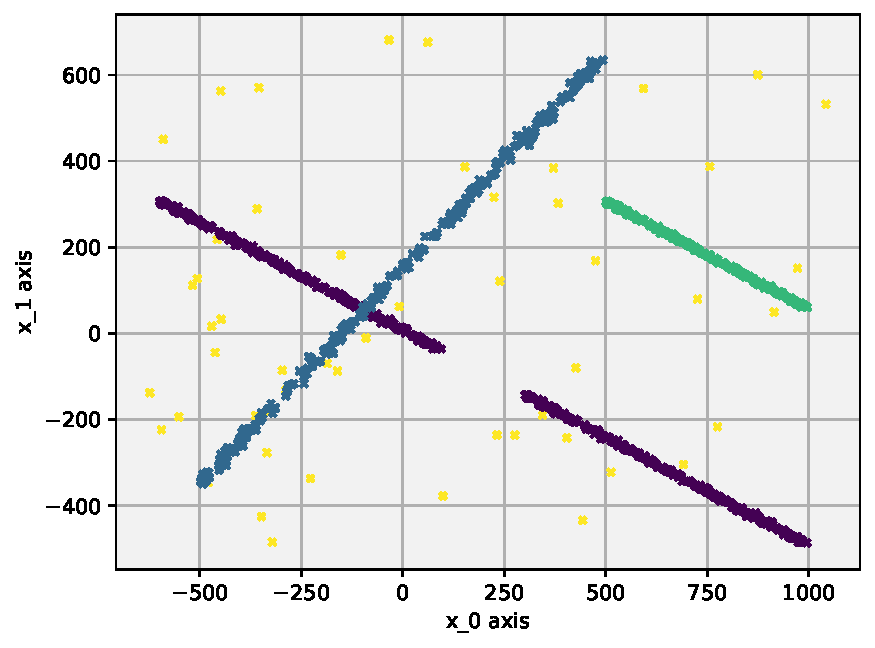
\includegraphics[width=\textwidth]{evalfigures/2DSetGrid.pdf}
    \captionof{figure}{Insight into clustering structure in 2D and 3D}
    \label{fig:my_label}
    \end{minipage}%
    \begin{minipage}[t]{.5\textwidth}
    \centering
    \captionsetup{width=.9\linewidth}
    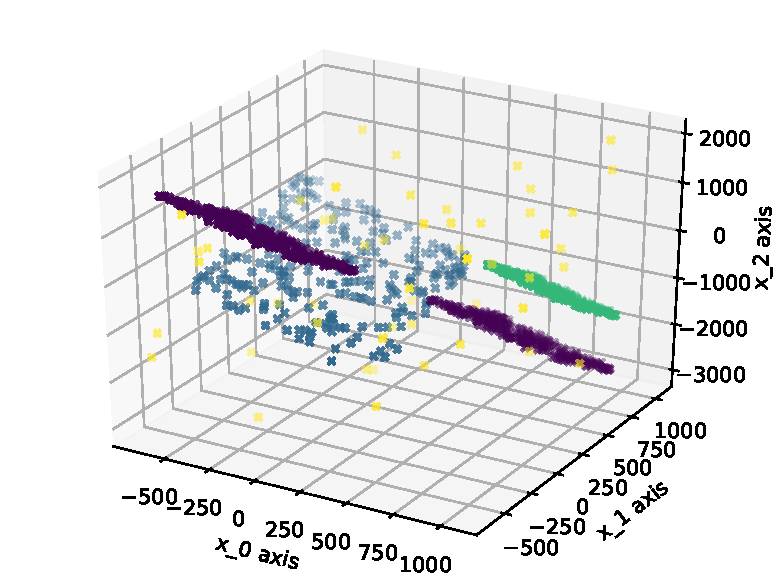
\includegraphics[width=\textwidth]{evalfigures/3DSet.pdf}
    \captionof{figure}{Insight into clustering structure in 2D and 3D}
    \label{fig:my_label}
    \end{minipage}%
\end{figure}

% The algorithms and evaluation are implemented in \textit{python v3.7.4}. Each of the data sets locally dense correlations are uniquely labeled and previously pruned noise points relabeled to a nearby linear correlation if the point was within a certain vicinity from the correlation away. For the density-based clustering we applied \gls{optics} from \textit{scikit-learn v0.21.2}\cite{pedregosa2011scikit} and for the extraction of the correlations we utilized \gls{cash} from the data mining tool \textit{\gls{elki} v0.7.5}\cite{achtert2008elki}. 

% (which data sets have been used? How many data objects? How many clusters? Which programming language and libraries? On which hardware?) [0.5]
\section{Performance}
 To evaluate the performance of our algorithm compared to \gls{cash} we performed up to 500 iterations of random parameter search on each data set while tracking runtime for a measure of efficiency and scoring the effectivity based on the \gls{ari} and \gls{nmi} score compared to our prelabeled groundtruth. However due to time constraints we bounded the maximal time for all iterations to a maximum of 24 hours. \todor{unsicher ob das rein soll}We’d like to note at this point that the current implementation may not satisfy the need to deliver a high performance with regards to the runtime, since we rely on \gls{elki}, which temporarily stores our necessary intermediate results to disk and therefore bottlenecks on I/O. For future work, we recommend to further research and elaborate on strategies to accelerate the execution time of our approach. 
 
\begin{table}[hb]
\centering
\resizebox{\textwidth}{!}{%
\begin{tabular}{@{}llll@{}}
\toprule
Test setting           & Dimensions & Noise in \% & \# of objects \\ \midrule
Increasing objects    & 3D         & 5           & -             \\
Increasing dimensions & -          & 5           & 10000         \\
Increasing noise      & 3D         & -           & 10000         \\ \bottomrule
\end{tabular}%
}
\caption{}
\label{tab:reducedsetup}
\end{table}
 
\subsection{Efficiency}
In context of efficiency we investigate the runtime performance of both local (our algorithm) and global (default \gls{cash}) by three different indications, namely number of objects, number of dimensions and amount of noise.

For the first aspect, we increased the data sets with regards to the number of objects. Here, we asked deliberately: what is the impact regarding the runtime if we modify the data set size?
And further: do we observe any differences between the original \gls{cash} algorithm and our approach? In theory we expect that our method yields similar results as \gls{cash}.

%  The evaluation of runtime performance measures the average runtime of the three different settings for both local (our algorithm) and global (default \gls{cash}) approaches. 

\begin{figure}[h]
    \centering
    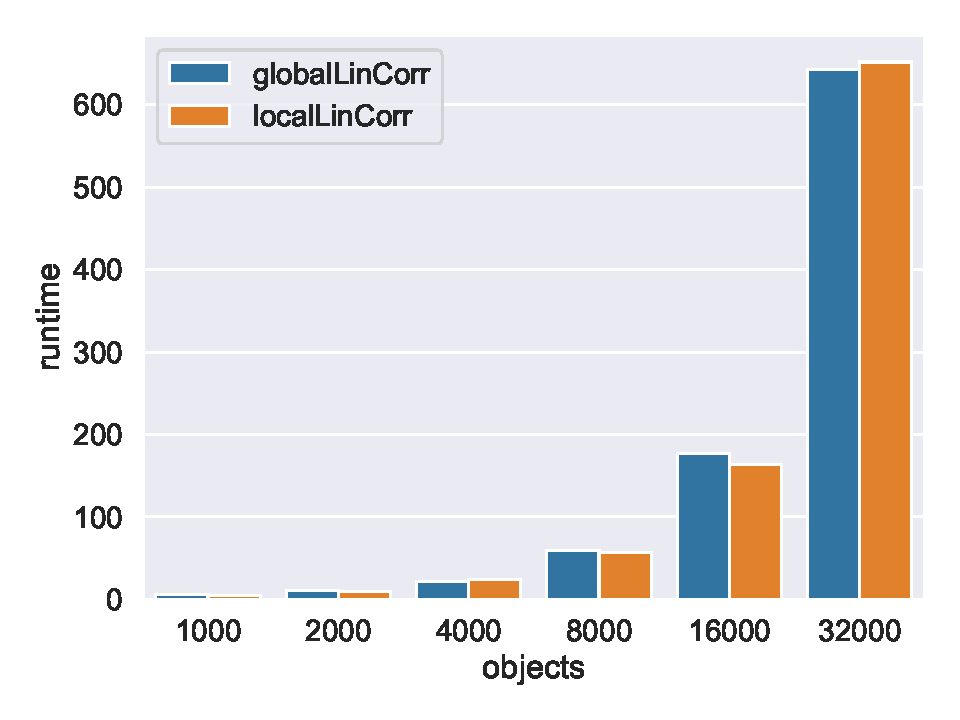
\includegraphics[width=0.8\textwidth]{evaluation/per_objects/Avg_Runtime_3D_N5_pobjects_bar.pdf}
    \caption{Caption}
    \label{fig:eval_per_objects}   
\end{figure}

\autoref{fig:eval_per_objects} shows the average runtime of both algorithms w.r.t. the \textit{number of objects} in 3-dimensional clusters of the data set. The data sets had a variable size of 1000, 2000, 4000, 8000, 16000 and 32000 number of objects with 5 percent noise respective to the data set size. Here our algorithm scales comparably to \gls{cash} and does not deteriorate in runtime performance even with higher numbers of objects even though the overhead of the partitioning, stitching and relabeling increases. This can be explained due to the shorter runtimes of the localized \gls{cash} processes, since the partitioning step reduces the amount of regions of interest in the parameter space of the Hough transform.\\

The second question regarding to efficiency is: How fast does our algorithm perform at different levels of noise? Is it comparable to the original \gls{cash}?. To assess the robustness of our algorithms efficiency against noise we compared the average runtimes of 500 iterations of both algorithms with respect to the amount of noise in the data space. Instead of modifying the total number of points of the whole data set, we now just evaluate the impact of different levels of noise percentage and compare the results of our approach with \gls{cash}s.

% of the average runtime w.r.t the different dimensionalities of the data space is depicted in \autoref{fig:eval_per_dim}.

\begin{figure}[h]
    \centering
        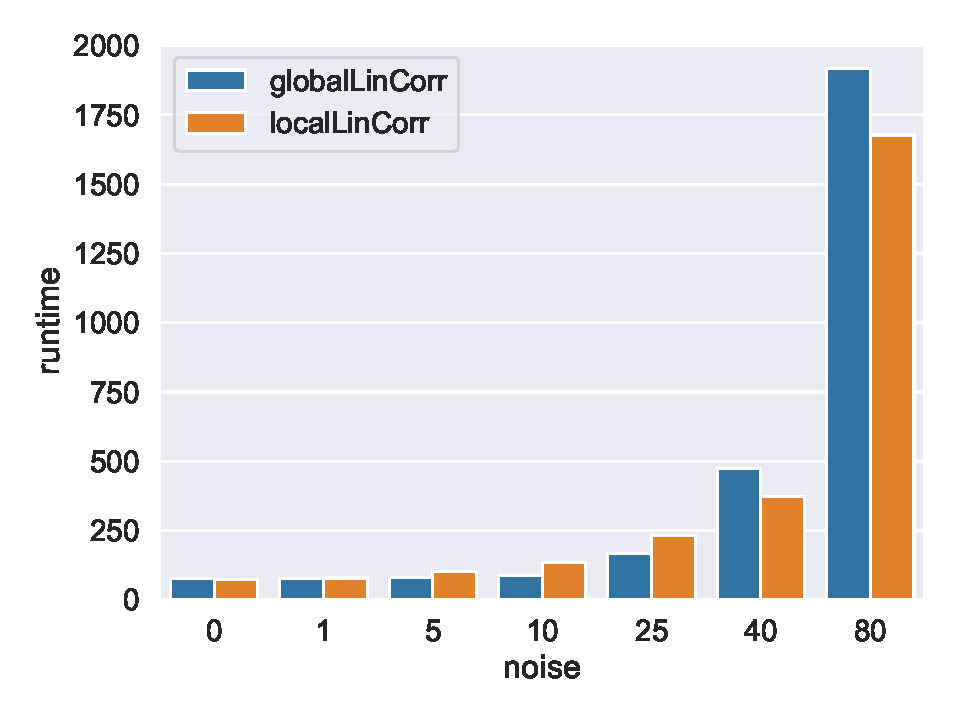
\includegraphics[width=0.8\textwidth]{evaluation/per_noise/Avg_Runtime_3D_O10000_pnoise_bar.pdf}
    \caption{Runtime in seconds w.r.t. the noise percentage}
    \label{fig:eval_per_noise}
\end{figure}

\autoref{fig:eval_per_noise} shows the average runtime of our algorithm with respect to the noise percentage of the data sets compared to the global approach. In this experiment our algorithms were evaluated on a 3-dimensional data set with 10000 points distributed among all clusters and seven different levels of noise percentage (0,1,5,10,25,40,80) on top of the initial data set. Note that noise points close enough to existing correlation clusters are relabeled to the respective cluster before evaluation which slightly skews the actual noise percentage in each data set.
As in the previous runtime measurements with regards to number of objects, the runtimes with respect to noise also remain stable on multiple levels compared to the global \gls{cash}. The overhead of the other components again is compensated by the quicker runtime of the partitioned \gls{cash}. At higher levels of noise (40 and 80 percent) it is even noticeable, that our approach gets a slight speed up compared to the global approach, since at these levels of noise the global cash will need to process more candidates in parameter space. In comparison our approach prunes away density-based noise first due to the partitioning step and leaves each localized \gls{cash} with comparably less candidates.
% At very low levels of noise both algorithms runtime remain stable. However increasing the noise further creates a gap in runtime results in favor of the global approach. This might be due to the overhead of the components increasing faster compared to the reduction in runtime of \gls{cash}, and second 

Our last runtime evaluation was conducted with regards to the dimensionality of the data set. Unlike in previous experiments, the data sets now change in \textit{space} instead of number of data objects. To keep a consistent comparable setting between the dimensionalities, we enforce our data set to be composed of similar four characteristic correlations, building a data space with partially split, intersecting and parallel $d-1$-dimensional hyperplanes. 
Note that runtimes dependent on dimensionality scale in $\mathcal{O}(2^d)$. Therefore the runtime figure with respect to the dimensionality scales logarithmically on the y-axis. Due to time constraints we set an upper bound for the runtime and restricted each run to a maximum of two hours. \todor{soll das rein?}

\begin{figure}[h]
    \centering
        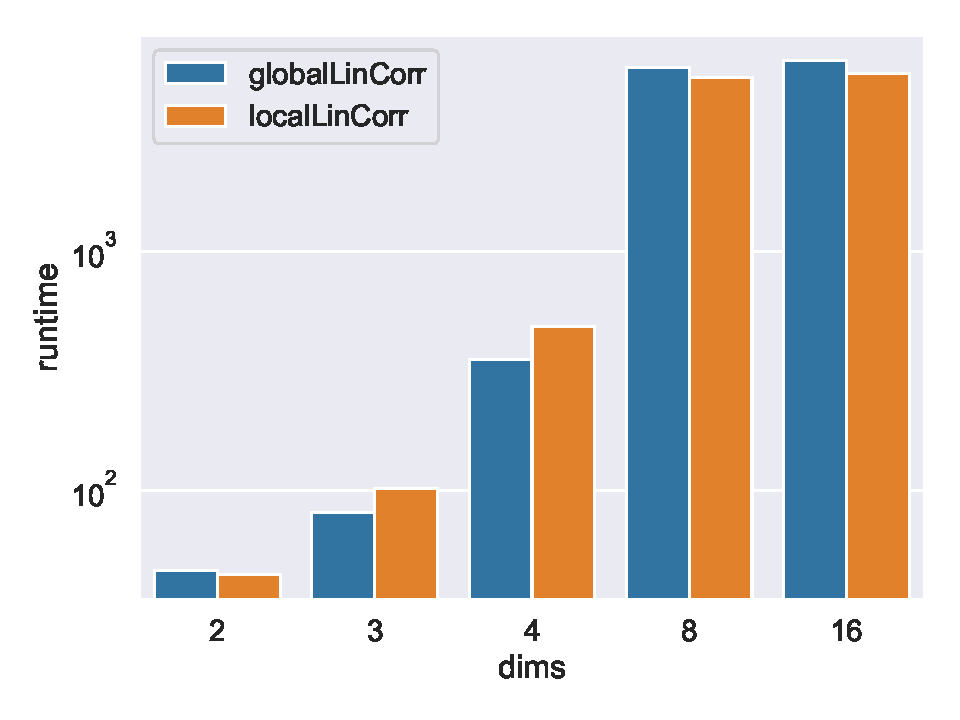
\includegraphics[width=0.8\textwidth]{evaluation/per_dims/Avg_Runtime_O10000_N5_pdims_log.pdf}
    \caption{Runtime in seconds w.r.t. the dimensionality of the whole data set - lower is better}
    \label{fig:eval_per_dims}
\end{figure}

\autoref{fig:eval_per_dims} shows a comparison of local and global algorithms average runtime performances with regards to expanding dimensionalities. This experiment was ran on data sets with 10000 objects and 5 percent noise with 2,3,4,8 and 16 dimensions. As expected the average runtime corresponding to the increasing dimensionality increases exponentially for both approaches, considering the runtime complexity of \gls{cash} and our algorithms complexity, which is also dominated by the complexity of \gls{cash}s $\mathcal{O}(2^d)$. Therefore it is sensible that both algorithms again perform comparably.
Since we capped the maximum runtime of each parameter search iteration to 2 hours we observe a stagnation of the runtime at 16 dimensions.\\

Summarized the experiments have demonstrated that the average runtime of our local approach is closely comparable to the default \gls{cash} with respect to number of points, amount of noise and dimensionalities. Therefore as assumed the overhead produced by the preprocessing component \gls{optics} and the postprocessing components \textit{Stitching} and \textit{Relabeling} are compensated by the faster runtime of the localized \gls{cash} ran on the partitioned subinterval of the data space. 
 
\subsection{Effectiveness}
To measure the clustering performance measures we picked the best parameter sets of the previous 500 iterations of parameter search of the efficiency evaluation for both local and global approach and stacked their \gls{ari} and \gls{nmi} scores up against each other. 

In our first setting we compared \gls{cash} and our algorithm according to the best \gls{ari} and \gls{nmi} scorings achieved during the parameter search with regards to the variable number of objects in data space. 
\begin{figure}[h]
    \centering
    \begin{minipage}[t]{.5\textwidth}
      \centering  
      \captionsetup{width=.9\linewidth}
      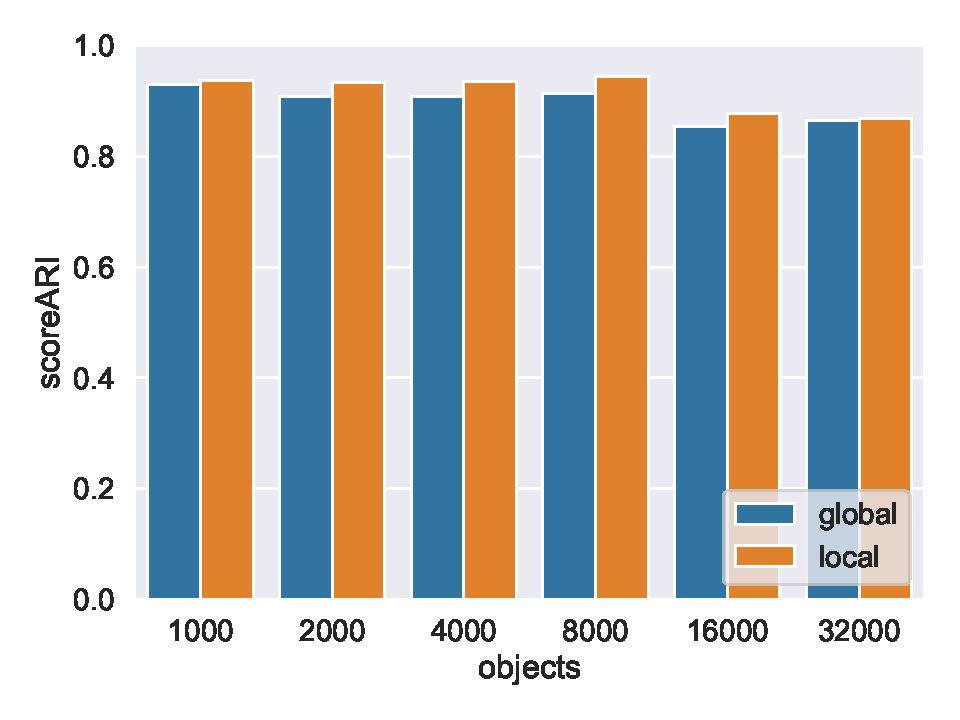
\includegraphics[width=\textwidth]{evaluation/per_objects/Best_ARI_3D_N5_pobjects_bar.pdf}
      \captionsetup{labelformat=empty}
      \caption{\gls{ari} score}
      \label{fig:ariperpts}
    \end{minipage}%
    \begin{minipage}[t]{.5\textwidth}
      \centering
      \captionsetup{width=.9\linewidth}
      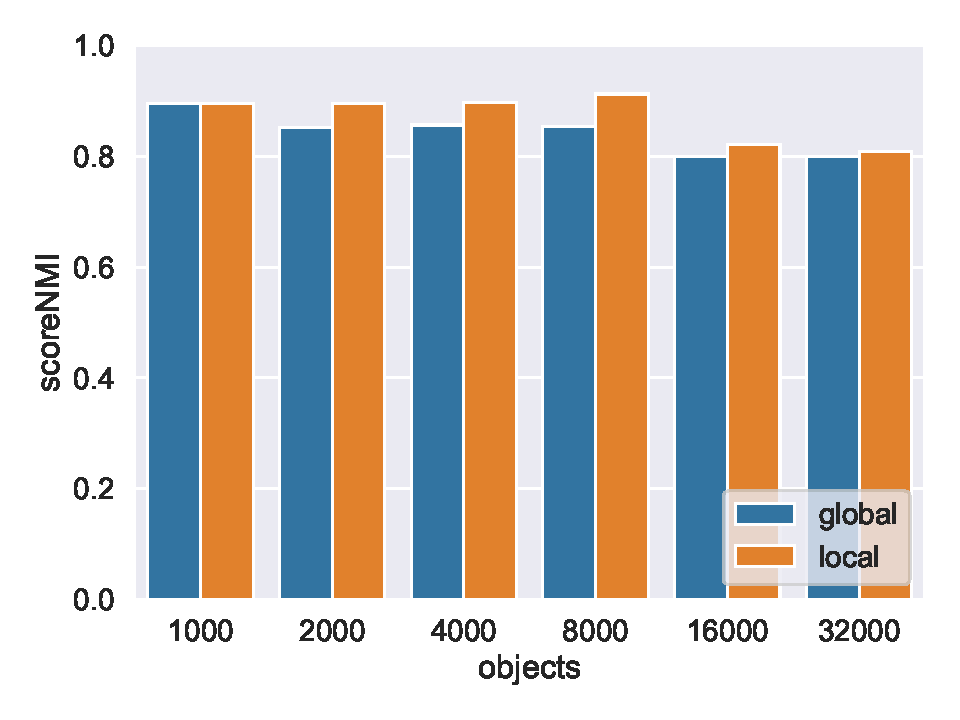
\includegraphics[width=\textwidth]{evaluation/per_objects/Best_NMI_3D_N5_pobjects_bar.pdf}
      \captionsetup{labelformat=empty}
      \caption{\gls{nmi} score}
      \label{fig:nmiperpts}
    \end{minipage}
    \caption{Scoring w.r.t the number of objects - higher is better}
    \label{fig:scoreperpts}
\end{figure}

\autoref{fig:scoreperpts} shows the comparison of the clustering scores achieved by both the local and global approach on the 3-dimensional data set with 5 percent noise with respect to six variable numbers of objects (1000, 2000, 4000, 8000, 16000, 32000). In terms of cluster size both algorithms perform comparably and score a similar \gls{ari} and \gls{nmi} score of over $0.8$. 

To assess the robustness of our clustering algorithm against noise, the second clustering performance evaluation was conducted on a data set with variable levels of noise. Given the best parameter settings achieved during the 500 iterations of parameter search in the efficiency evaluation step, we compared the \gls{ari} and the \gls{nmi} scores at different levels of noise of both algorithms against each other.
\begin{figure}[h]
    \centering
    \begin{minipage}[t]{.5\textwidth}
      \centering  
      \captionsetup{width=.9\linewidth}
      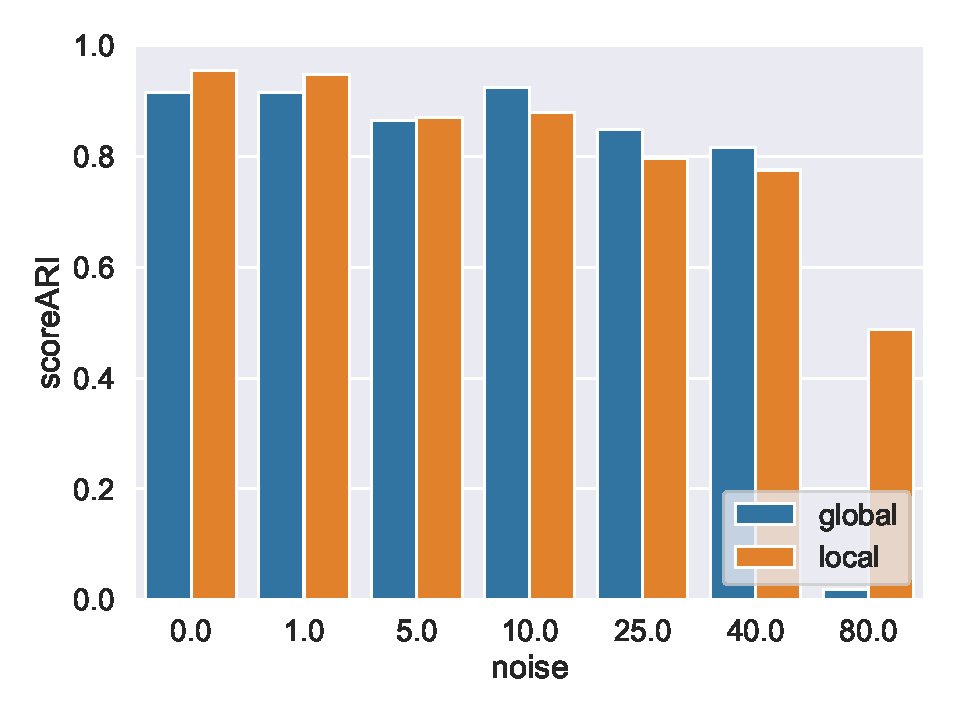
\includegraphics[width=\textwidth]{evaluation/per_noise/Best_ARI_3D_O10000_pnoise_bar.pdf}
      \captionof{figure}{\gls{ari} score w.r.t. amount of noise}
      \label{fig:ariperpts}
    \end{minipage}%
    \begin{minipage}[t]{.5\textwidth}
      \centering
      \captionsetup{width=.9\linewidth}
      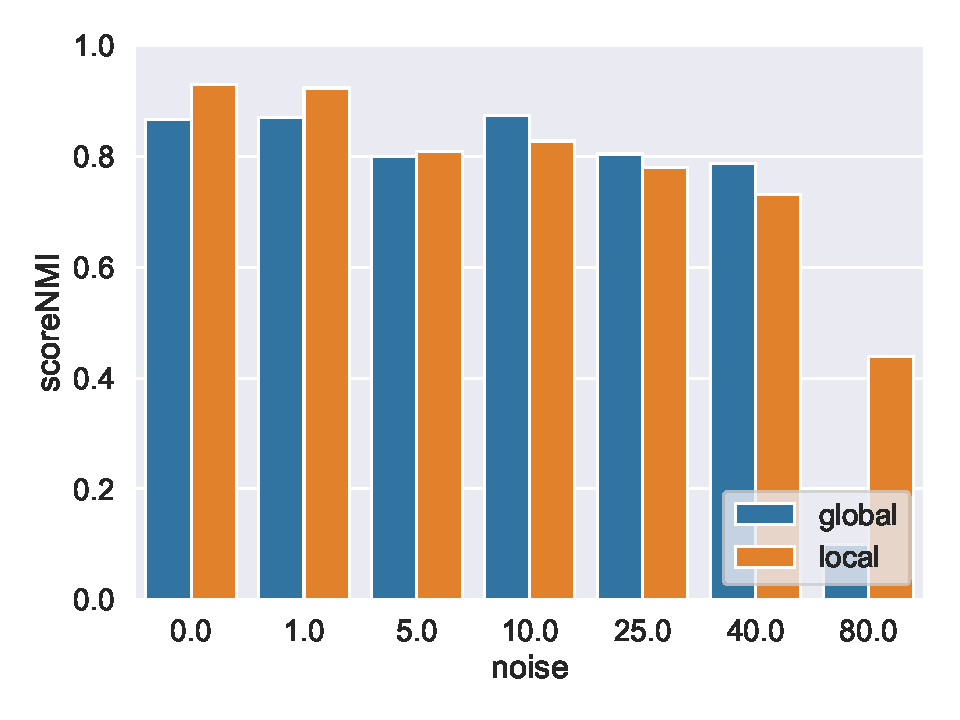
\includegraphics[width=\textwidth]{evaluation/per_noise/Best_NMI_3D_O10000_pnoise_bar.pdf}
      \captionof{figure}{\gls{nmi} score w.r.t. amount of noise}
      \label{fig:nmiperpts}
    \end{minipage}    
    \caption{Scoring w.r.t the noise percentage - higher is better}
    \label{fig:scorepernoise}
\end{figure}
The second experiment was ran on 3-dimensional base data sets with 10000 data points spread among all clusters with seven varying amounts of noise (0,1,5,10,25,40,80).
As \autoref{fig:scorepernoise} shows, the results of the clustering performance evaluation scoring between our algorithm and \gls{cash} remains close to eachother for low to mid levels of noise. At 80 percent noise our algorithm performs even better than the global \gls{cash}. This could be due to the high percentage of noise creating a high amount of candidate cells in parameter space, which are all considered as valid correlations in the global \gls{cash}. In contrast our approaches preprocessing via \gls{optics} might extract the underlying correlations, which are characterized by comparably more dense regions, first and and extract those local correlations via \gls{cash} faster and more accurately, since the partitions contain less noise and therefore the parameter space less candidates. These few prominent local correlations are then stitched together if similar enough and previously not considered points are relabeled, all together resulting in an quicker and more accurate global clustering compared to default \gls{cash} itself.

Our last clustering performance evaluation was targeted at the impact of the dimensionality of the data set. Here, we again picked the best parameter sets previously obtained during the runtime assessment to compare our algorithm with \gls{cash}.
\begin{figure}[h]
    \centering
    \begin{minipage}[t]{.5\textwidth}
      \centering  
      \captionsetup{width=.9\linewidth}
      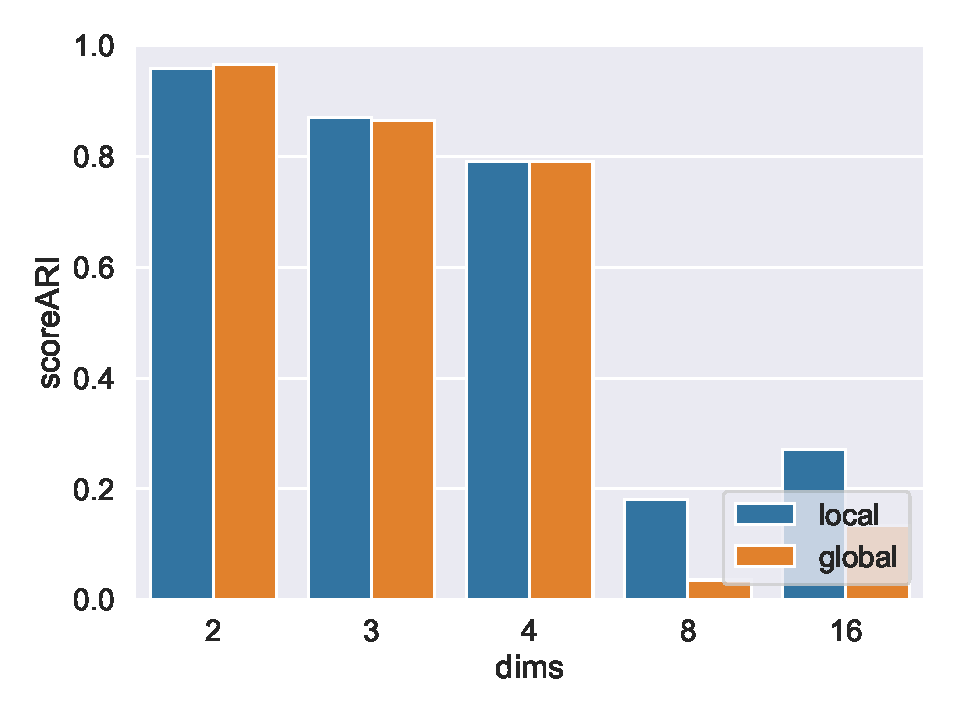
\includegraphics[width=\textwidth]{evaluation/per_dims/Best_ARI_O10000_N5_pdims_bar.pdf}
      \captionof{figure}{\gls{ari} score w.r.t. dimensionality}
      \label{fig:ariperpts}
    \end{minipage}%
    \begin{minipage}[t]{.5\textwidth}
      \centering
      \captionsetup{width=.9\linewidth}
      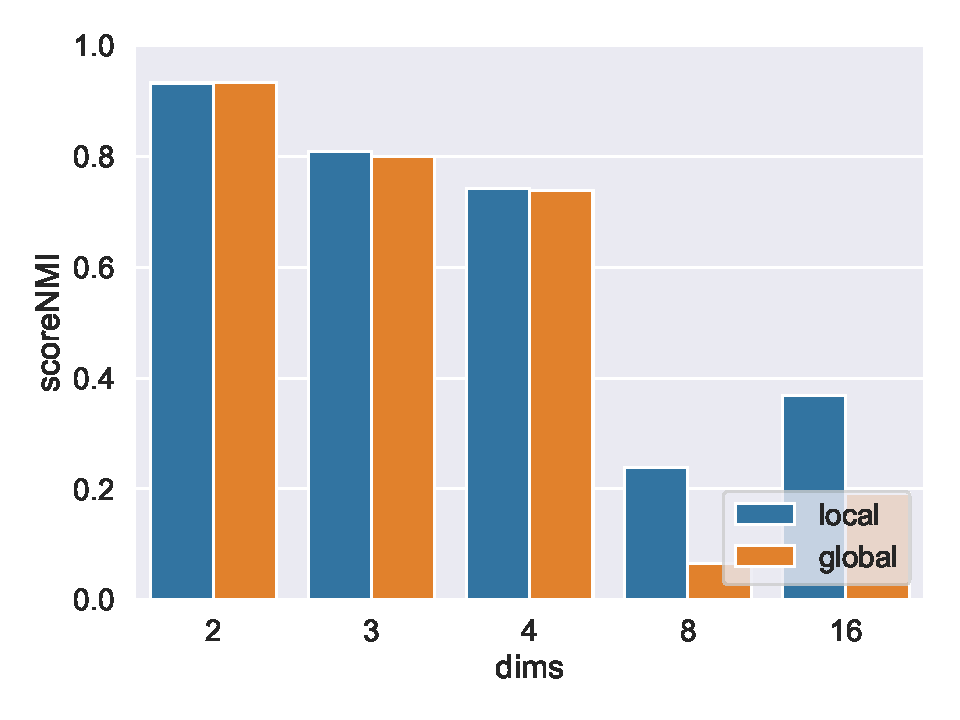
\includegraphics[width=\textwidth]{evaluation/per_dims/Best_NMI_O10000_N5_pdims_bar.pdf}
      \captionof{figure}{\gls{nmi} score w.r.t. dimensionality}
      \label{fig:nmiperpts}
    \end{minipage}
    \caption{Scoring w.r.t the dimensionality - higher is better}
    \label{fig:scoreperdims}
\end{figure}

\autoref{fig:scoreperdims} shows the different scores, \gls{ari} and \gls{nmi}, between both global and local approach applied on data sets with a fixed amount of 10000 data objects and 5 percent noise and a variable dimensionality of 2,3,4,8 and 16.
Note that since the evaluation of the runtime performance with regards to 8 and 16 dimensional data sets were stopped early due to time constraints, the optimal scorings of both 8 and 16 dimensional data sets are not representative for the optimal scores and will not be considered. 
The results of dimensions 2,3 and 4 show similar clustering results compared to both algorithms, however as the direction over these dimensions \gls{ari} and \gls{nmi} scores suggest, both \gls{cash} and our algorithm have an downwards trend in terms of clustering score with regards to dimensionality. This might be due to the fact, that the search space for \gls{cash} increases exponentially with respect to the dimensions, which increases the possible regions of interest (c.f. \autoref{fig:cash3d}). Instead of a single intersection in a point as a region of interest in 2-dimensional space, a 3-dimensional space for comparison has a complex curve as intersection which increases the amount of regions of interest considerably. This increased complexity might be the reason for the deteriorating performance in increasing dimensions. \todor{erwaehnt orginal cash das deswegen nicht?}\\

Summarized our experiments show, that our local approach yields similar results in various settings in terms of runtime as well as in terms of clustering performance compared to the original \gls{cash}, with an additional benefit of detecting locally dense correlations. \autoref{fig:clusterexample} shows an example of our algorithm with the local correlations clustering as an intermediate result and the relabeled global view of the correlation clustering. \autoref{fig:gclusterexample} shows the equivalent clustering performed by the default \gls{cash}. \todor{kann laenger sein}

\begin{figure}
    \centering
    \includegraphics{}
    \caption{Caption}
    \label{fig:clusterexample}
\end{figure}

\begin{figure}
    \centering
    \includegraphics{}
    \caption{Caption}
    \label{fig:gclusterexample}
\end{figure}

% \section{Parameters available and their impacts}
% As our algorithm depends on many components such as \gls{optics} and \gls{cash} which come with several parameters themselves. In this section we discuss their meaning and their impact for the clustering results.

% \subsection{Metrics: CosineSimiliarity(n1,n2), CosineSimiliarity(n1,n2) + EuclidianDistance(d) [2-3]}

% \subsection{Median vs.  Mean}

% \section{Results between Dense approach with stitching and Global approach}

% \section{Test on real world data set(s) [1]}

% %evtl. "Hyperparameter sensitivity" d.h. wie 'empfindlich' ist das verfahren bzgl. welchen Parameter Einstellungen?